\documentclass[11pt,a4paper]{article}
\usepackage[utf8]{inputenc}
\usepackage[T1]{fontenc}
\usepackage[spanish,es-nodecimaldot]{babel}
\usepackage{lmodern}
\usepackage{amsmath,amssymb}
\usepackage{graphicx}
\usepackage{booktabs,array,tabularx}
\usepackage{xcolor}
\usepackage{tcolorbox}
\usepackage{fancyhdr}
\usepackage{enumitem}
\usepackage{geometry}
\usepackage{hyperref}
\usepackage{caption}
\usepackage{float}
\usepackage{siunitx}
\usepackage{microtype}
\geometry{left=2.0cm,right=2.0cm,top=2.1cm,bottom=2.1cm}
\sisetup{output-decimal-marker={,},per-mode=symbol}
\definecolor{azulutn}{RGB}{24,55,94}
\definecolor{azulclaro}{RGB}{238,246,255}
\definecolor{verde}{RGB}{15,118,110}
\definecolor{amarillo}{RGB}{181,101,29}
\definecolor{rojocaja}{RGB}{164,58,58}
\hypersetup{colorlinks=true,linkcolor=azulutn,urlcolor=azulutn}
\pagestyle{fancy}
\fancyhf{}
\lhead{Física Aplicada a la Tecnología de Alimentos}
\rhead{Unidad 4 - Trabajo y Energía}
\cfoot{\thepage}
\setlength{\headheight}{14pt}
\setlist[itemize]{leftmargin=1.4em,itemsep=2pt,topsep=4pt}
\setlist[enumerate]{leftmargin=1.6em,itemsep=3pt,topsep=4pt}
\newtcolorbox{metodo}{colback=azulclaro,colframe=azulutn,title=Modelo de resolución,fonttitle=\bfseries}
\newtcolorbox{resultado}{colback=green!5,colframe=verde,title=Resultado,fonttitle=\bfseries}
\newtcolorbox{validacion}{colback=yellow!7,colframe=amarillo,title=Validación y control,fonttitle=\bfseries}
\newtcolorbox{alerta}{colback=red!4,colframe=rojocaja,title=Observación sobre la respuesta de la guía,fonttitle=\bfseries}
\newcommand{\vect}[1]{\vec{#1}}
\newcommand{\dif}{\,\mathrm{d}}

\begin{document}

\begin{titlepage}
\centering
\begin{minipage}{0.18\textwidth}\centering

\includegraphics[width=0.72\linewidth]{figuras/logo_utn.png}
\end{minipage}\hfill
\begin{minipage}{0.58\textwidth}\centering
{\Large \textbf{Universidad Tecnológica Nacional}}\\[2mm]
{\large Facultad Regional La Plata}\\[1mm]
{\large Física Aplicada a la Tecnología de Alimentos}
\end{minipage}\hfill
\begin{minipage}{0.18\textwidth}\centering

\includegraphics[width=0.85\linewidth]{figuras/logo_ciab.jpg}
\end{minipage}

\vfill
{\Huge\bfseries Guía de ejercicios resueltos\par}
\vspace{4mm}
{\LARGE Unidad 4: Trabajo y Energía\par}
\vspace{5mm}
{\large Fuerzas conservativas y disipativas - Teorema trabajo--energía - Conservación de la energía - Potencia\par}
\vspace{12mm}
\begin{tcolorbox}[width=.88\textwidth,colback=azulclaro,colframe=azulutn]
\centering
Ejercicios desarrollados del Trabajo Práctico N.º 06: \\
\textbf{3, 4, 6, 8, 10, 17, 19, 22--23 (integrados), 27 y 29.}
\end{tcolorbox}
\vfill
{\large Material de resolución docente - 2026\par}
\end{titlepage}

\tableofcontents
\newpage

\section{Criterios de resolución y validación}
Esta guía toma como base el \textit{Trabajo Práctico N.º 06: Trabajo y Energía. Fuerzas conservativas y disipativas. Teorema de Trabajo y Energía. Principio de Conservación de la Energía}. Se adopta, salvo indicación contraria,
\[
 g=\SI{9.8}{m/s^2}.
\]

En cada problema se utiliza la siguiente secuencia:
\begin{enumerate}
\item \textbf{Sistema en estudio y estados inicial/final.}
\item \textbf{Hipótesis simplificativas:} modelo de partícula cuando corresponde, superficies lisas o rugosas según el enunciado, resortes ideales, ausencia de resistencia del aire y referencia de energía potencial explícita.
\item \textbf{Interacciones relevantes:} fuerza aplicada, peso, normal, rozamiento y fuerza elástica.
\item \textbf{Modelo físico:} definición de trabajo, teorema trabajo--energía o balance de energía mecánica.
\item \textbf{Resolución matemática y control dimensional.}
\item \textbf{Validación:} comparación con la respuesta incluida en el TP y análisis de coherencia física.
\end{enumerate}

\begin{validacion}
La revisión detallada detecta inconsistencias en algunas respuestas impresas del TP. En particular, los ejercicios 4, 8, 23 y 29 requieren observaciones. En esta guía se conserva el planteo original, pero se informa el resultado que surge de un cálculo física y algebraicamente consistente.
\end{validacion}

\section{Ejercicio 3 - Trabajo de fuerzas sobre un desplazamiento horizontal}
\textbf{Enunciado resumido.} Un bloque de \SI{15}{kg} se desplaza \SI{5}{m} horizontalmente. Una fuerza de \SI{70}{N} forma \(20^\circ\) con la horizontal. Se pide el trabajo de la fuerza aplicada, de la normal y del peso.

\begin{metodo}
Sistema: el bloque. El desplazamiento es horizontal. Para una fuerza constante,
\[
W=F\,d\cos\theta.
\]
El trabajo depende de la componente de la fuerza paralela al desplazamiento.
\end{metodo}

\subsection*{a) Trabajo de la fuerza aplicada}
\[
W_F=(\SI{70}{N})(\SI{5}{m})\cos20^\circ
=\SI{328.89}{J}\approx\SI{329}{J}.
\]

\subsection*{b) Trabajo de la normal}
La normal es perpendicular al desplazamiento:
\[
W_N=N\,d\cos90^\circ=0.
\]

\subsection*{c) Trabajo del peso}
El peso también es perpendicular al desplazamiento:
\[
W_g=mg\,d\cos90^\circ=0.
\]

\begin{resultado}
\[
\boxed{W_F\approx\SI{329}{J}},\qquad
\boxed{W_N=0},\qquad
\boxed{W_g=0}.
\]
\end{resultado}

\begin{validacion}
Coincide con la respuesta del TP. La mención de superficie rugosa implica que podría existir rozamiento, pero el problema no pide ese trabajo ni proporciona \(\mu\); por lo tanto no puede obtenerse el trabajo total sólo con los datos dados.
\end{validacion}

\section{Ejercicio 4 - Trabajo de una fuerza variable y teorema trabajo--energía}
\textbf{Enunciado resumido.} Un cuerpo de \SI{2}{kg} se mueve sobre una superficie lisa. Una fuerza horizontal varía con la posición de acuerdo con la gráfica original. Antes de actuar la fuerza el cuerpo lleva \SI{10}{m/s}. Luego entra en una superficie rugosa y finalmente se detiene.

\begin{figure}[H]
\centering
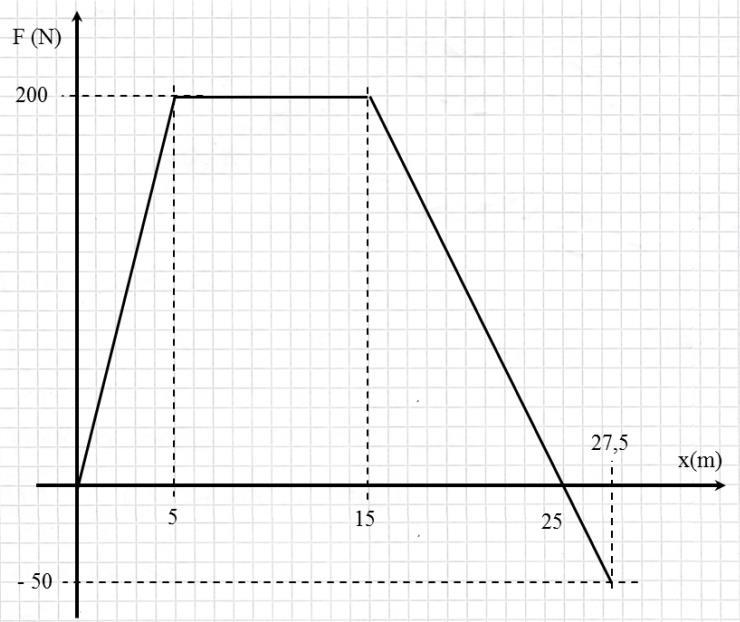
\includegraphics[width=.72\textwidth]{figuras/ex04_grafico_original.png}
\caption{Gráfica original \(F(x)\) del ejercicio 4.}
\end{figure}

\begin{metodo}
Para una fuerza variable colineal con el desplazamiento,
\[
W=\int F(x)\dif x,
\]
que geométricamente es el área algebraica bajo la curva. Luego se aplica el teorema trabajo--energía:
\[
W_{\mathrm{neto}}=\Delta K.
\]
\end{metodo}

\subsection*{a) Trabajo de la fuerza variable}
La gráfica se descompone en cuatro áreas:
\begin{align*}
A_1&=\frac12(5)(200)=\SI{500}{J},\\
A_2&=(10)(200)=\SI{2000}{J},\\
A_3&=\frac12(10)(200)=\SI{1000}{J},\\
A_4&=-\frac12(2.5)(50)=-\SI{62.5}{J}.
\end{align*}
Por tanto,
\[
W=A_1+A_2+A_3+A_4=\boxed{\SI{3437.5}{J}}.
\]

\subsection*{b) Velocidad al finalizar la acción de la fuerza}
La energía cinética inicial es
\[
K_i=\frac12(2)(10)^2=\SI{100}{J}.
\]
En el tramo liso, peso y normal no realizan trabajo, de modo que
\[
K_f=K_i+W=100+3437.5=\SI{3537.5}{J}.
\]
Entonces
\[
v_f=\sqrt{\frac{2K_f}{m}}=\boxed{\SI{59.48}{m/s}}.
\]
El valor \SI{60}{m/s} del TP es una aproximación por redondeo.

\subsection*{c) Fuerzas en el tramo rugoso}
Una vez que deja de actuar el agente exterior, actúan el peso, la normal y el rozamiento cinético. Como el desplazamiento es horizontal,
\[
W_g=0,\qquad W_N=0.
\]

\subsection*{d) Trabajo de cada agente hasta detenerse}
Al ingresar al tramo rugoso el bloque tiene \(K_i'=\SI{3537.5}{J}\); al detenerse, \(K_f'=0\). Por lo tanto,
\[
W_{\mathrm{neto}}=0-3537.5=-\SI{3537.5}{J}.
\]
El único agente que realiza trabajo es el rozamiento:
\[
\boxed{W_{fr}=-\SI{3537.5}{J}},\qquad W_N=0,\qquad W_g=0.
\]

\begin{alerta}
El TP imprime \(W_{fr}=-\SI{100}{J}\). Ese valor coincide en magnitud con la energía cinética inicial, antes de actuar la fuerza variable, y no con la energía cinética al entrar al tramo rugoso. El balance correcto exige \(-\SI{3537.5}{J}\), o aproximadamente \(-\SI{3600}{J}\) si antes se redondea \(v_f\) a \SI{60}{m/s}.
\end{alerta}

\section{Ejercicio 6 - Lanzamiento vertical y conservación de la energía}
\textbf{Datos:} \(m=\SI{20}{kg}\), \(v_0=\SI{50}{m/s}\), \(U=0\) en la superficie terrestre.

\begin{metodo}
Se desprecia la resistencia del aire. Durante el vuelo sólo actúa el peso, que es conservativo. Por ello,
\[
E_m=K+U_g=\frac12mv^2+mgh=\text{constante}.
\]
\end{metodo}

\subsection*{a) Energías iniciales}
\[
K_0=\frac12(20)(50)^2=\boxed{\SI{25000}{J}},\qquad U_0=0,
\]
\[
E_0=\boxed{\SI{25000}{J}}.
\]

\subsection*{b) Después de \SI{3}{s}}
\[
v_3=50-9.8(3)=\SI{20.6}{m/s},
\]
\[
h_3=50(3)-\frac12(9.8)(3)^2=\SI{105.9}{m}.
\]
Así,
\[
K_3=\frac12(20)(20.6)^2=\boxed{\SI{4243.6}{J}},
\]
\[
U_3=(20)(9.8)(105.9)=\boxed{\SI{20756.4}{J}},
\]
\[
E_3=K_3+U_3=\boxed{\SI{25000}{J}}.
\]

\subsection*{c) A \SI{100}{m}}
\[
U_{100}=20(9.8)(100)=\boxed{\SI{19600}{J}},
\]
\[
K_{100}=25000-19600=\boxed{\SI{5400}{J}}.
\]
Como verificación,
\[
v_{100}=\sqrt{\frac{2(5400)}{20}}=\SI{23.24}{m/s}.
\]

\subsection*{d) Altura cuando \(K\) se reduce un 80\%}
Queda el 20\% de la energía cinética inicial:
\[
K=0.20K_0=\SI{5000}{J}.
\]
Entonces
\[
U=25000-5000=\SI{20000}{J},
\]
\[
h=\frac{20000}{20(9.8)}=\boxed{\SI{102.04}{m}}.
\]

\begin{validacion}
Los resultados coinciden con los valores del TP, salvo diferencias de redondeo. En todos los estados \(K+U=\SI{25000}{J}\), que constituye el control físico principal.
\end{validacion}

\section{Ejercicio 8 - Trabajo neto y trabajo del rozamiento}
\textbf{Datos:} \(d=\SI{1.2}{m}\), \(F=\SI{49}{N}\), \(W_{\mathrm{tot}}=\SI{47.04}{J}\).

\subsection*{a) Trabajo de la fuerza aplicada}
\[
W_F=Fd=(49)(1.2)=\boxed{\SI{58.8}{J}}.
\]

\subsection*{b) Trabajo del rozamiento}
Peso y normal no realizan trabajo, de modo que
\[
W_{\mathrm{tot}}=W_F+W_{fr}.
\]
Por lo tanto,
\[
W_{fr}=47.04-58.8=\boxed{-\SI{11.76}{J}}.
\]

\begin{alerta}
En la clave impresa aparece \(+\SI{11.76}{J}\). El signo debe ser negativo: el rozamiento se opone al movimiento y el trabajo total es menor que el trabajo positivo de la fuerza aplicada.
\end{alerta}

\section{Ejercicio 10 - Trabajo de varias fuerzas en un plano inclinado}
\textbf{Datos:} \(m=\SI{4}{kg}\), \(\alpha=20^\circ\), \(s=\SI{20}{m}\), \(F_1=\SI{80}{N}\) horizontal, \(F_2=\SI{100}{N}\) paralela al plano. Plano liso.

\begin{figure}[H]
\centering
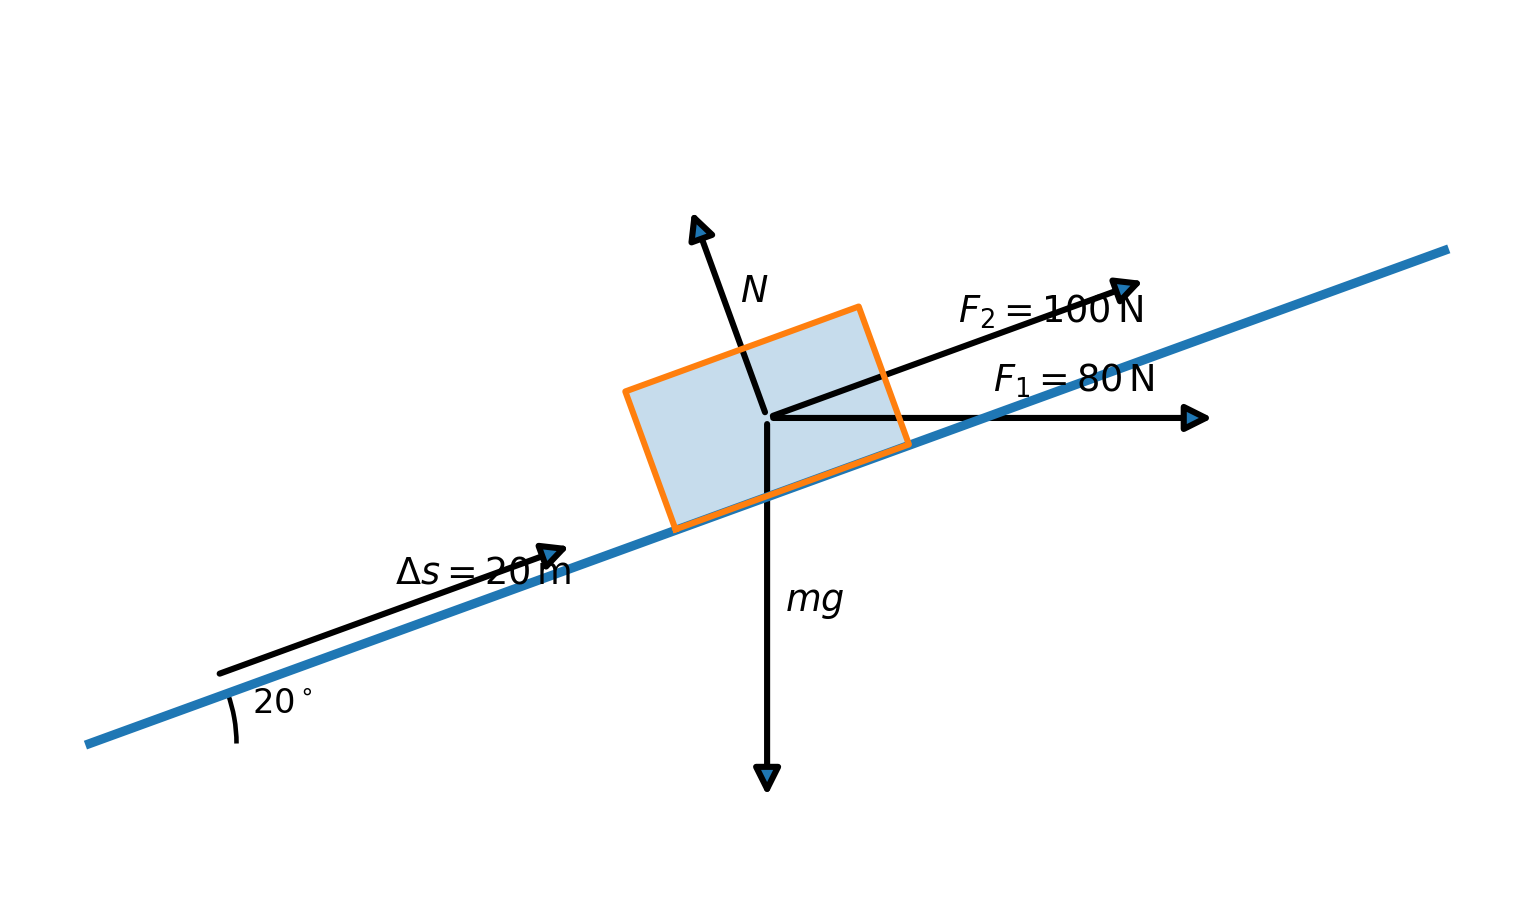
\includegraphics[width=.75\textwidth]{figuras/ex10_plano_inclinado.png}
\caption{Esquema de fuerzas para el ejercicio 10.}
\end{figure}

\begin{metodo}
El trabajo total es la suma escalar de los trabajos. La normal no realiza trabajo. El peso realiza trabajo negativo durante el ascenso.
\end{metodo}

Para la fuerza horizontal,
\[
W_1=F_1s\cos20^\circ
=80(20)\cos20^\circ
=\boxed{\SI{1503.5}{J}}.
\]
Para la fuerza paralela al plano,
\[
W_2=F_2s=100(20)=\boxed{\SI{2000}{J}}.
\]
El trabajo del peso es
\[
W_g=-mg(s\sin20^\circ)
=-4(9.8)(20)\sin20^\circ
=\boxed{-\SI{268.14}{J}}.
\]
La normal es perpendicular al movimiento:
\[
W_N=0.
\]
Por lo tanto,
\[
W_{\mathrm{tot}}=1503.5+2000-268.14
=\boxed{\SI{3235.36}{J}}.
\]

\begin{validacion}
Coincide con la guía: \(W_1\approx\SI{1504}{J}\), \(W_2=\SI{2000}{J}\), \(W_g\approx-\SI{268}{J}\) y \(W_{\mathrm{tot}}\approx\SI{3235}{J}\).
\end{validacion}

\section{Ejercicio 17 - Resorte y disipación por rozamiento}
\textbf{Datos:} \(m=\SI{1}{kg}\), \(k=\SI{120}{N/m}\), compresión inicial \(x_1=\SI{0.15}{m}\). El bloque parte del reposo y termina nuevamente en reposo.

\begin{figure}[H]
\centering
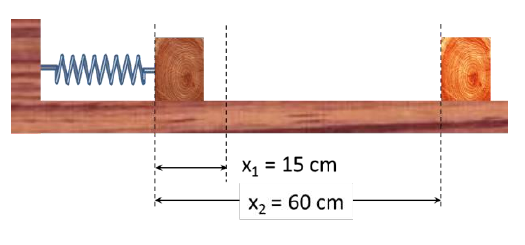
\includegraphics[width=.72\textwidth]{figuras/ex17_original.png}
\caption{Figura original del TP para el ejercicio 17.}
\end{figure}

\begin{metodo}
Sistema bloque--resorte. La energía inicial es potencial elástica; la energía final es nula. La disminución de energía mecánica es igual al trabajo del rozamiento.
\end{metodo}

\[
E_i=U_{e,i}=\frac12kx_1^2
=\frac12(120)(0.15)^2
=\SI{1.35}{J}.
\]
Al detenerse con el resorte sin deformación,
\[
E_f=0.
\]
Usando
\[
E_i+W_{fr}=E_f,
\]
se obtiene
\[
\boxed{W_{fr}=-\SI{1.35}{J}}.
\]

\begin{validacion}
Coincide con el TP. El signo negativo expresa disipación. El valor \(x_2\) no es necesario para hallar el trabajo total mediante energía; sí sería necesario para calcular una fuerza media de rozamiento.
\end{validacion}

\section{Ejercicio 19 - Pista, rozamiento localizado y resorte}
\textbf{Datos:} \(m=\SI{10}{kg}\), \(h=\SI{3}{m}\), rozamiento sólo en \(BC\), \(k=\SI{2250}{N/m}\), compresión máxima \(x=\SI{0.30}{m}\). El bloque parte y termina momentáneamente en reposo.

\begin{figure}[H]
\centering
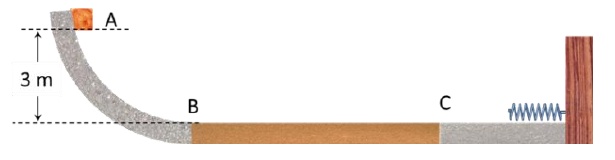
\includegraphics[width=.86\textwidth]{figuras/ex19_original.png}
\caption{Figura original del TP para el ejercicio 19.}
\end{figure}

\begin{metodo}
Entre el estado inicial en \(A\) y la máxima compresión del resorte, el único trabajo no conservativo es el rozamiento en \(BC\):
\[
E_i+W_{fr}=E_f.
\]
\end{metodo}

En \(A\),
\[
K_i=0,\qquad U_{g,i}=mgh=10(9.8)(3)=\SI{294}{J}.
\]
En la máxima compresión,
\[
K_f=0,\qquad U_{g,f}=0,
\]
\[
U_{e,f}=\frac12kx^2
=\frac12(2250)(0.30)^2
=\SI{101.25}{J}.
\]
Por tanto,
\[
294+W_{fr}=101.25,
\]
\[
\boxed{W_{fr}=-\SI{192.75}{J}}.
\]

\begin{validacion}
Coincide exactamente con la respuesta del TP. La diferencia \(294-101.25=192.75\,\mathrm{J}\) es la energía mecánica transformada por rozamiento en \(BC\).
\end{validacion}

\section{Ejercicios 22 y 23 integrados - Resorte y rulo vertical}
Se tratan como una única situación progresiva: primero se obtiene la compresión crítica para completar el rulo sin perder contacto y luego se incorpora rozamiento y valores numéricos.

\begin{figure}[H]
\centering
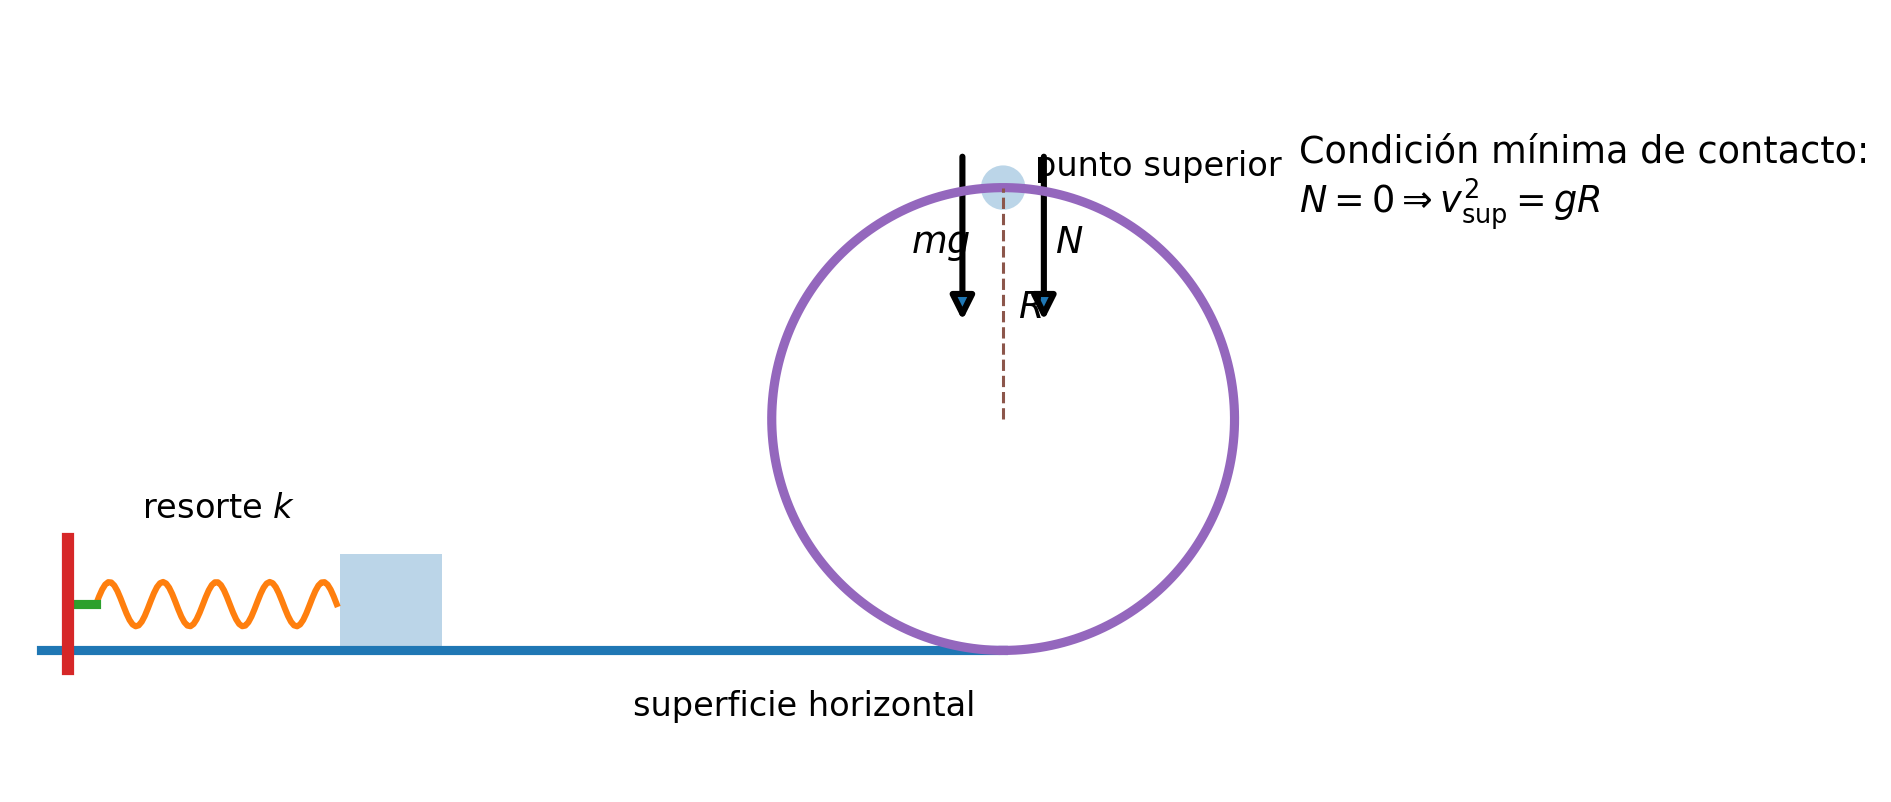
\includegraphics[width=.92\textwidth]{figuras/ex22_23_loop_vertical.png}
\caption{Modelo utilizado para los ejercicios 22--23.}
\end{figure}

\subsection{Parte A - Compresión crítica del resorte (ejercicio 22)}
\begin{metodo}
En el punto superior, la condición límite para conservar el contacto es \(N=0\). Allí el peso debe proporcionar toda la aceleración centrípeta.
\end{metodo}

\[
mg=\frac{mv_{\mathrm{sup}}^2}{R}
\quad\Longrightarrow\quad
v_{\mathrm{sup}}^2=gR.
\]
Conservando energía desde el resorte hasta la cima:
\[
\frac12k(\Delta x)^2
=mg(2R)+\frac12mv_{\mathrm{sup}}^2.
\]
Sustituyendo \(v_{\mathrm{sup}}^2=gR\):
\[
\frac12k(\Delta x)^2
=2mgR+\frac12mgR
=\frac52mgR.
\]
Luego,
\[
\boxed{(\Delta x)_c=\sqrt{\frac{5mgR}{k}}}.
\]

\begin{validacion}
Coincide con la expresión del TP. Físicamente es la \textbf{compresión mínima o crítica} para completar el rulo manteniendo contacto; una compresión mayor también permite alcanzar la parte superior.
\end{validacion}

\subsection{Parte B - Superficie rugosa y compresión doble (ejercicio 23)}
Datos: \(m=\SI{5}{kg}\), \(k=\SI{1000}{N/m}\), \(R=\SI{5}{m}\), \(x=2x_c\). El trabajo de roce es el 10\% de la energía elástica inicial.

\[
x_c=\sqrt{\frac{5(5)(5)(9.8)}{1000}}=\SI{1.1068}{m},
\qquad x=\SI{2.2136}{m}.
\]
La energía elástica inicial es
\[
U_{e,i}=\frac12kx^2=\SI{2450}{J}.
\]
El rozamiento realiza
\[
W_{fr}=-0.10U_{e,i}=-\SI{245}{J}.
\]
En la parte superior,
\[
U_{g,\mathrm{sup}}=mg(2R)=\SI{490}{J}.
\]
Balance energético:
\[
2450-245=K_{\mathrm{sup}}+490,
\]
\[
K_{\mathrm{sup}}=\SI{1715}{J}.
\]
Entonces,
\[
\frac12mv^2=1715
\quad\Longrightarrow\quad
\boxed{v_{\mathrm{sup}}=\SI{26.19}{m/s}}.
\]

En la cima, hacia el centro apuntan tanto el peso como la normal:
\[
mg+N=\frac{mv^2}{R}.
\]
Así,
\[
N=\frac{mv^2}{R}-mg
=\boxed{\SI{637}{N}}.
\]

\begin{alerta}
El TP informa \(v\approx\SI{26.5}{m/s}\) y \(F_{aro}=\SI{652.25}{N}\). La velocidad se aproxima a ese valor si se adopta \(g=\SI{10}{m/s^2}\). Sin redondeo intermedio, con \(g=10\) se obtiene \(v=\SI{26.46}{m/s}\) y \(N=\SI{650}{N}\). Con \(g=9.8\), coherente con la mayor parte del TP, los valores consistentes son \(26.19\,\mathrm{m/s}\) y \(637\,\mathrm{N}\).
\end{alerta}

\section{Ejercicio 27 - Trabajo y potencia en aceleración uniforme}
\textbf{Datos:} \(m=\SI{1500}{kg}\), \(v_i=0\), \(v_f=\SI{10}{m/s}\), \(\Delta t=\SI{3}{s}\). Se desprecia resistencia al avance.

\subsection*{a) Trabajo efectuado}
\[
W=\Delta K=\frac12mv_f^2
=\frac12(1500)(10)^2
=\boxed{\SI{75000}{J}}.
\]

\subsection*{b) Potencia promedio}
\[
P_{\mathrm{prom}}=\frac{W}{\Delta t}
=\frac{75000}{3}
=\boxed{\SI{25000}{W}}=\boxed{\SI{25.0}{kW}}.
\]

\subsection*{c) Potencia instantánea en \(t=\SI{2}{s}\)}
\[
a=\frac{10}{3}=\SI{3.333}{m/s^2},
\]
\[
F=ma=1500\left(\frac{10}{3}\right)=\SI{5000}{N}.
\]
A los \SI{2}{s},
\[
v=at=\frac{10}{3}(2)=\SI{6.667}{m/s}.
\]
Por tanto,
\[
P=Fv=(5000)(6.667)
=\boxed{\SI{33333}{W}}\approx\boxed{\SI{33.3}{kW}}.
\]

\begin{validacion}
Coincide con el TP. La potencia instantánea aumenta con el tiempo porque la fuerza motriz se mantiene constante mientras la velocidad crece.
\end{validacion}

\section{Ejercicio 29 - Potencia necesaria para una bomba}
\textbf{Enunciado resumido.} Una bomba eleva \SI{200}{L} de agua por minuto desde \SI{6}{m} de profundidad y la descarga a \SI{9}{m/s}.

\begin{figure}[H]
\centering
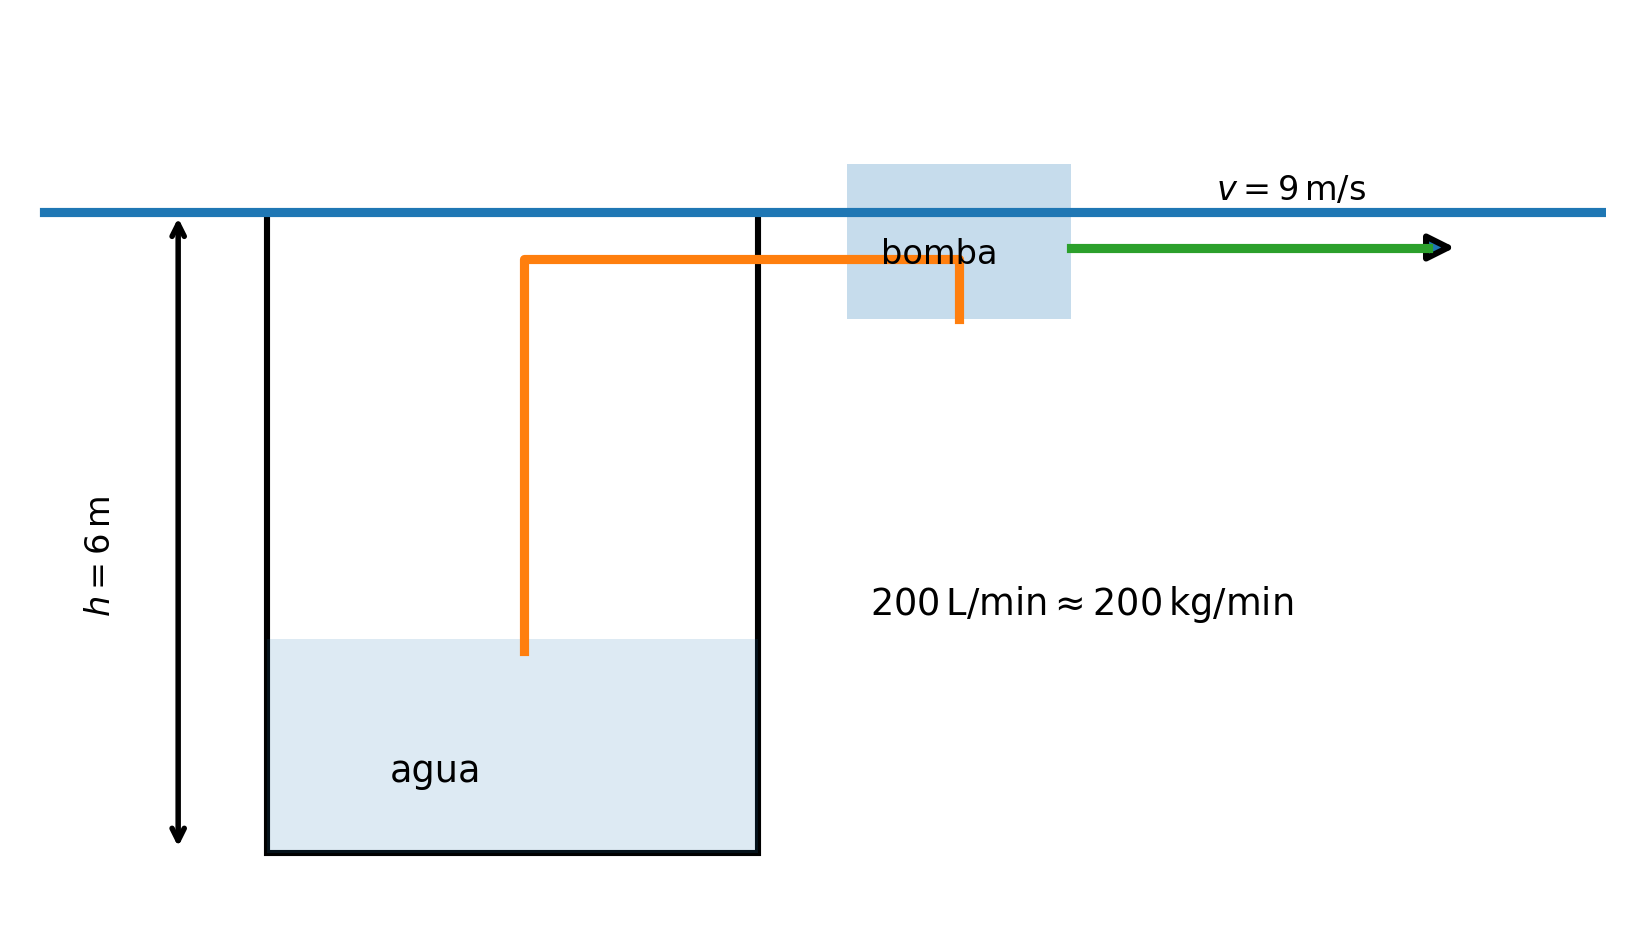
\includegraphics[width=.78\textwidth]{figuras/ex29_bomba.png}
\caption{Modelo energético para la bomba del ejercicio 29.}
\end{figure}

\begin{metodo}
Se toma \(\rho_{agua}\approx\SI{1000}{kg/m^3}\). Por tanto, \SI{200}{L}=\SI{0.200}{m^3} $\approx$ \SI{200}{kg}. En un minuto la bomba aporta energía potencial gravitatoria y energía cinética al agua. Se desprecia toda pérdida porque no se proporciona rendimiento.
\end{metodo}

\subsection*{a) Trabajo por minuto para elevar el agua}
\[
W_g=mgh=(200)(9.8)(6)
=\boxed{\SI{11760}{J}}.
\]

\subsection*{b) Energía cinética adquirida}
\[
\Delta K=\frac12mv^2
=\frac12(200)(9)^2
=\boxed{\SI{8100}{J}}.
\]

\subsection*{c) Potencia mecánica ideal}
La energía total entregada por minuto es
\[
E_{\mathrm{min}}=11760+8100=\SI{19860}{J/min}.
\]
Entonces,
\[
P=\frac{19860}{60}
=\boxed{\SI{331}{W}}
=\boxed{\SI{0.331}{kW}}.
\]
Si el conjunto bomba--motor tuviera rendimiento global \(\eta\), la potencia de entrada sería
\[
P_{\mathrm{entrada}}=\frac{331}{\eta}\ \mathrm{W}.
\]

\begin{alerta}
El TP indica aproximadamente \(\SI{0.2}{kW}\). Ese valor corresponde prácticamente a \(mgh/60\) y omite la energía cinética necesaria para descargar el agua a \SI{9}{m/s}. Como el inciso (b) pide explícitamente esa energía y el inciso (c) solicita la potencia necesaria para cumplir ambas condiciones, el resultado ideal coherente es \(\SI{0.331}{kW}\).
\end{alerta}


\end{document}
